\documentclass[1p]{elsarticle_modified}
%\bibliographystyle{elsarticle-num}

%\usepackage[colorlinks]{hyperref}
%\usepackage{abbrmath_seonhwa} %\Abb, \Ascr, \Acal ,\Abf, \Afrak
\usepackage{amsfonts}
\usepackage{amssymb}
\usepackage{amsmath}
\usepackage{amsthm}
\usepackage{scalefnt}
\usepackage{amsbsy}
\usepackage{kotex}
\usepackage{caption}
\usepackage{subfig}
\usepackage{color}
\usepackage{graphicx}
\usepackage{xcolor} %% white, black, red, green, blue, cyan, magenta, yellow
\usepackage{float}
\usepackage{setspace}
\usepackage{hyperref}

\usepackage{tikz}
\usetikzlibrary{arrows}

\usepackage{multirow}
\usepackage{array} % fixed length table
\usepackage{hhline}

%%%%%%%%%%%%%%%%%%%%%
\makeatletter
\renewcommand*\env@matrix[1][\arraystretch]{%
	\edef\arraystretch{#1}%
	\hskip -\arraycolsep
	\let\@ifnextchar\new@ifnextchar
	\array{*\c@MaxMatrixCols c}}
\makeatother %https://tex.stackexchange.com/questions/14071/how-can-i-increase-the-line-spacing-in-a-matrix
%%%%%%%%%%%%%%%

\usepackage[normalem]{ulem}

\newcommand{\msout}[1]{\ifmmode\text{\sout{\ensuremath{#1}}}\else\sout{#1}\fi}
%SOURCE: \msout is \stkout macro in https://tex.stackexchange.com/questions/20609/strikeout-in-math-mode

\newcommand{\cancel}[1]{
	\ifmmode
	{\color{red}\msout{#1}}
	\else
	{\color{red}\sout{#1}}
	\fi
}

\newcommand{\add}[1]{
	{\color{blue}\uwave{#1}}
}

\newcommand{\replace}[2]{
	\ifmmode
	{\color{red}\msout{#1}}{\color{blue}\uwave{#2}}
	\else
	{\color{red}\sout{#1}}{\color{blue}\uwave{#2}}
	\fi
}

\newcommand{\Sol}{\mathcal{S}} %segment
\newcommand{\D}{D} %diagram
\newcommand{\A}{\mathcal{A}} %arc


%%%%%%%%%%%%%%%%%%%%%%%%%%%%%5 test

\def\sl{\operatorname{\textup{SL}}(2,\Cbb)}
\def\psl{\operatorname{\textup{PSL}}(2,\Cbb)}
\def\quan{\mkern 1mu \triangleright \mkern 1mu}

\theoremstyle{definition}
\newtheorem{thm}{Theorem}[section]
\newtheorem{prop}[thm]{Proposition}
\newtheorem{lem}[thm]{Lemma}
\newtheorem{ques}[thm]{Question}
\newtheorem{cor}[thm]{Corollary}
\newtheorem{defn}[thm]{Definition}
\newtheorem{exam}[thm]{Example}
\newtheorem{rmk}[thm]{Remark}
\newtheorem{alg}[thm]{Algorithm}

\newcommand{\I}{\sqrt{-1}}
\begin{document}

%\begin{frontmatter}
%
%\title{Boundary parabolic representations of knots up to 8 crossings}
%
%%% Group authors per affiliation:
%\author{Yunhi Cho} 
%\address{Department of Mathematics, University of Seoul, Seoul, Korea}
%\ead{yhcho@uos.ac.kr}
%
%
%\author{Seonhwa Kim} %\fnref{s_kim}}
%\address{Center for Geometry and Physics, Institute for Basic Science, Pohang, 37673, Korea}
%\ead{ryeona17@ibs.re.kr}
%
%\author{Hyuk Kim}
%\address{Department of Mathematical Sciences, Seoul National University, Seoul 08826, Korea}
%\ead{hyukkim@snu.ac.kr}
%
%\author{Seokbeom Yoon}
%\address{Department of Mathematical Sciences, Seoul National University, Seoul, 08826,  Korea}
%\ead{sbyoon15@snu.ac.kr}
%
%\begin{abstract}
%We find all boundary parabolic representation of knots up to 8 crossings.
%
%\end{abstract}
%\begin{keyword}
%    \MSC[2010] 57M25 
%\end{keyword}
%
%\end{frontmatter}

%\linenumbers
%\tableofcontents
%
\newcommand\colored[1]{\textcolor{white}{\rule[-0.35ex]{0.8em}{1.4ex}}\kern-0.8em\color{red} #1}%
%\newcommand\colored[1]{\textcolor{white}{ #1}\kern-2.17ex	\textcolor{white}{ #1}\kern-1.81ex	\textcolor{white}{ #1}\kern-2.15ex\color{red}#1	}

{\Large $\underline{12a_{0208}~(K12a_{0208})}$}

\setlength{\tabcolsep}{10pt}
\renewcommand{\arraystretch}{1.6}
\vspace{1cm}\begin{tabular}{m{100pt}>{\centering\arraybackslash}m{274pt}}
\multirow{5}{120pt}{
	\centering
	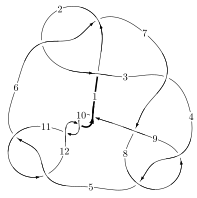
\includegraphics[width=112pt]{../../../GIT/diagram.site/Diagrams/png/1009_12a_0208.png}\\
\ \ \ A knot diagram\footnotemark}&
\allowdisplaybreaks
\textbf{Linearized knot diagam} \\
\cline{2-2}
 &
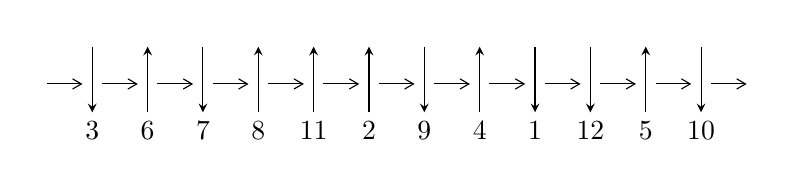
\begin{tikzpicture}[x=20pt, y=17pt]
	% nodes
	\node (C0) at (0, 0) {};
	\node (C1) at (1, 0) {};
	\node (C1U) at (1, +1) {};
	\node (C1D) at (1, -1) {3};

	\node (C2) at (2, 0) {};
	\node (C2U) at (2, +1) {};
	\node (C2D) at (2, -1) {6};

	\node (C3) at (3, 0) {};
	\node (C3U) at (3, +1) {};
	\node (C3D) at (3, -1) {7};

	\node (C4) at (4, 0) {};
	\node (C4U) at (4, +1) {};
	\node (C4D) at (4, -1) {8};

	\node (C5) at (5, 0) {};
	\node (C5U) at (5, +1) {};
	\node (C5D) at (5, -1) {11};

	\node (C6) at (6, 0) {};
	\node (C6U) at (6, +1) {};
	\node (C6D) at (6, -1) {2};

	\node (C7) at (7, 0) {};
	\node (C7U) at (7, +1) {};
	\node (C7D) at (7, -1) {9};

	\node (C8) at (8, 0) {};
	\node (C8U) at (8, +1) {};
	\node (C8D) at (8, -1) {4};

	\node (C9) at (9, 0) {};
	\node (C9U) at (9, +1) {};
	\node (C9D) at (9, -1) {1};

	\node (C10) at (10, 0) {};
	\node (C10U) at (10, +1) {};
	\node (C10D) at (10, -1) {12};

	\node (C11) at (11, 0) {};
	\node (C11U) at (11, +1) {};
	\node (C11D) at (11, -1) {5};

	\node (C12) at (12, 0) {};
	\node (C12U) at (12, +1) {};
	\node (C12D) at (12, -1) {10};
	\node (C13) at (13, 0) {};

	% arrows
	\draw[->,>={angle 60}]
	(C0) edge (C1) (C1) edge (C2) (C2) edge (C3) (C3) edge (C4) (C4) edge (C5) (C5) edge (C6) (C6) edge (C7) (C7) edge (C8) (C8) edge (C9) (C9) edge (C10) (C10) edge (C11) (C11) edge (C12) (C12) edge (C13) ;	\draw[->,>=stealth]
	(C1U) edge (C1D) (C2D) edge (C2U) (C3U) edge (C3D) (C4D) edge (C4U) (C5D) edge (C5U) (C6D) edge (C6U) (C7U) edge (C7D) (C8D) edge (C8U) (C9U) edge (C9D) (C10U) edge (C10D) (C11D) edge (C11U) (C12U) edge (C12D) ;
	\end{tikzpicture} \\
\hhline{~~} \\& 
\textbf{Solving Sequence} \\ \cline{2-2} 
 &
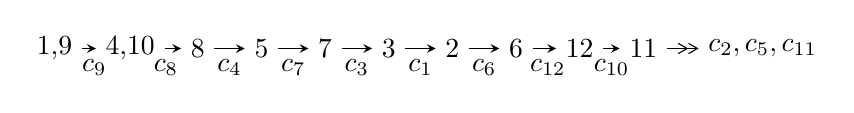
\begin{tikzpicture}[x=23pt, y=7pt]
	% node
	\node (A0) at (-1/8, 0) {1,9};
	\node (A1) at (17/16, 0) {4,10};
	\node (A2) at (17/8, 0) {8};
	\node (A3) at (25/8, 0) {5};
	\node (A4) at (33/8, 0) {7};
	\node (A5) at (41/8, 0) {3};
	\node (A6) at (49/8, 0) {2};
	\node (A7) at (57/8, 0) {6};
	\node (A8) at (65/8, 0) {12};
	\node (A9) at (73/8, 0) {11};
	\node (C1) at (1/2, -1) {$c_{9}$};
	\node (C2) at (13/8, -1) {$c_{8}$};
	\node (C3) at (21/8, -1) {$c_{4}$};
	\node (C4) at (29/8, -1) {$c_{7}$};
	\node (C5) at (37/8, -1) {$c_{3}$};
	\node (C6) at (45/8, -1) {$c_{1}$};
	\node (C7) at (53/8, -1) {$c_{6}$};
	\node (C8) at (61/8, -1) {$c_{12}$};
	\node (C9) at (69/8, -1) {$c_{10}$};
	\node (A10) at (11, 0) {$c_{2},c_{5},c_{11}$};

	% edge
	\draw[->,>=stealth]	
	(A0) edge (A1) (A1) edge (A2) (A2) edge (A3) (A3) edge (A4) (A4) edge (A5) (A5) edge (A6) (A6) edge (A7) (A7) edge (A8) (A8) edge (A9) ;
	\draw[->>,>={angle 60}]	
	(A9) edge (A10);
\end{tikzpicture} \\ 

\end{tabular} \\

\footnotetext{
The image of knot diagram is generated by the software ``\textbf{Draw programme}" developed by Andrew Bartholomew(\url{http://www.layer8.co.uk/maths/draw/index.htm\#Running-draw}), where we modified some parts for our purpose(\url{https://github.com/CATsTAILs/LinksPainter}).
}\phantom \\ \newline 
\centering \textbf{Ideals for irreducible components\footnotemark of $X_{\text{par}}$} 
 
\begin{align*}
I^u_{1}&=\langle 
-73876195581 u^{31}+635182095531 u^{30}+\cdots+1260543449654 b-1153435624046,\\
\phantom{I^u_{1}}&\phantom{= \langle  }-324186211813 u^{31}+2767349300228 u^{30}+\cdots+2521086899308 a+292251319739,\\
\phantom{I^u_{1}}&\phantom{= \langle  }u^{32}-8 u^{31}+\cdots-3 u+4\rangle \\
I^u_{2}&=\langle 
-46 u^{26} a+785 u^{26}+\cdots+710 a-2547,\;2 u^{26} a-2 u^{26}+\cdots-7 a+10,\;u^{27}-7 u^{26}+\cdots-2 u+1\rangle \\
I^u_{3}&=\langle 
b- u+1,\;a-1,\;u^2- u+1\rangle \\
I^u_{4}&=\langle 
b^2+1,\;u^2+a- u+2,\;u^3- u^2+2 u-1\rangle \\
\\
\end{align*}
\raggedright * 4 irreducible components of $\dim_{\mathbb{C}}=0$, with total 94 representations.\\
\footnotetext{All coefficients of polynomials are rational numbers. But the coefficients are sometimes approximated in decimal forms when there is not enough margin.}
\newpage
\renewcommand{\arraystretch}{1}
\centering \section*{I. $I^u_{1}= \langle -7.39\times10^{10} u^{31}+6.35\times10^{11} u^{30}+\cdots+1.26\times10^{12} b-1.15\times10^{12},\;-3.24\times10^{11} u^{31}+2.77\times10^{12} u^{30}+\cdots+2.52\times10^{12} a+2.92\times10^{11},\;u^{32}-8 u^{31}+\cdots-3 u+4 \rangle$}
\flushleft \textbf{(i) Arc colorings}\\
\begin{tabular}{m{7pt} m{180pt} m{7pt} m{180pt} }
\flushright $a_{1}=$&$\begin{pmatrix}0\\u\end{pmatrix}$ \\
\flushright $a_{9}=$&$\begin{pmatrix}1\\0\end{pmatrix}$ \\
\flushright $a_{4}=$&$\begin{pmatrix}0.128590 u^{31}-1.09768 u^{30}+\cdots+5.24512 u-0.115923\\0.0586066 u^{31}-0.503895 u^{30}+\cdots-1.40068 u+0.915030\end{pmatrix}$ \\
\flushright $a_{10}=$&$\begin{pmatrix}1\\u^2\end{pmatrix}$ \\
\flushright $a_{8}=$&$\begin{pmatrix}0.0983513 u^{31}-0.889506 u^{30}+\cdots+3.00247 u+0.618797\\0.0740836 u^{31}-0.470529 u^{30}+\cdots-1.24670 u+0.527414\end{pmatrix}$ \\
\flushright $a_{5}=$&$\begin{pmatrix}0.146540 u^{31}-1.26945 u^{30}+\cdots+4.04903 u+0.702930\\0.0976318 u^{31}-0.820411 u^{30}+\cdots-1.76926 u+1.02768\end{pmatrix}$ \\
\flushright $a_{7}=$&$\begin{pmatrix}0.172435 u^{31}-1.36004 u^{30}+\cdots+1.75577 u+1.14621\\0.0740836 u^{31}-0.470529 u^{30}+\cdots-1.24670 u+0.527414\end{pmatrix}$ \\
\flushright $a_{3}=$&$\begin{pmatrix}0.131853 u^{31}-1.12891 u^{30}+\cdots+1.57311 u+0.851141\\-0.0194438 u^{31}+0.129136 u^{30}+\cdots-1.66352 u+0.689740\end{pmatrix}$ \\
\flushright $a_{2}=$&$\begin{pmatrix}-0.0569748 u^{31}+0.488280 u^{30}+\cdots-2.43533 u+0.0685016\\-0.0390252 u^{31}+0.316515 u^{30}+\cdots+0.368581 u-0.112645\end{pmatrix}$ \\
\flushright $a_{6}=$&$\begin{pmatrix}0.256919 u^{31}-2.15298 u^{30}+\cdots+3.47300 u+0.998503\\0.136486 u^{31}-0.905042 u^{30}+\cdots-2.46312 u+0.976685\end{pmatrix}$ \\
\flushright $a_{12}=$&$\begin{pmatrix}u\\u^3+u\end{pmatrix}$ \\
\flushright $a_{11}=$&$\begin{pmatrix}u^2+1\\u^4+2 u^2\end{pmatrix}$\\&\end{tabular}
\flushleft \textbf{(ii) Obstruction class $= -1$}\\~\\
\flushleft \textbf{(iii) Cusp Shapes $= \frac{204288482497}{630271724827} u^{31}-\frac{1674264130767}{630271724827} u^{30}+\cdots+\frac{8358771694435}{630271724827} u+\frac{744767795870}{630271724827}$}\\~\\
\newpage\renewcommand{\arraystretch}{1}
\flushleft \textbf{(iv) u-Polynomials at the component}\newline \\
\begin{tabular}{m{50pt}|m{274pt}}
Crossings & \hspace{64pt}u-Polynomials at each crossing \\
\hline $$\begin{aligned}c_{1},c_{7}\end{aligned}$$&$\begin{aligned}
&u^{32}+15 u^{31}+\cdots+6 u+1
\end{aligned}$\\
\hline $$\begin{aligned}c_{2},c_{4},c_{6}\\c_{8}\end{aligned}$$&$\begin{aligned}
&u^{32}- u^{31}+\cdots+3 u^2+1
\end{aligned}$\\
\hline $$\begin{aligned}c_{3}\end{aligned}$$&$\begin{aligned}
&u^{32}+4 u^{31}+\cdots+192 u+128
\end{aligned}$\\
\hline $$\begin{aligned}c_{5},c_{11}\end{aligned}$$&$\begin{aligned}
&u^{32}+2 u^{31}+\cdots-3 u+2
\end{aligned}$\\
\hline $$\begin{aligned}c_{9},c_{10},c_{12}\end{aligned}$$&$\begin{aligned}
&u^{32}+8 u^{31}+\cdots+3 u+4
\end{aligned}$\\
\hline
\end{tabular}\\~\\
\newpage\renewcommand{\arraystretch}{1}
\flushleft \textbf{(v) Riley Polynomials at the component}\newline \\
\begin{tabular}{m{50pt}|m{274pt}}
Crossings & \hspace{64pt}Riley Polynomials at each crossing \\
\hline $$\begin{aligned}c_{1},c_{7}\end{aligned}$$&$\begin{aligned}
&y^{32}+11 y^{31}+\cdots+2 y+1
\end{aligned}$\\
\hline $$\begin{aligned}c_{2},c_{4},c_{6}\\c_{8}\end{aligned}$$&$\begin{aligned}
&y^{32}+15 y^{31}+\cdots+6 y+1
\end{aligned}$\\
\hline $$\begin{aligned}c_{3}\end{aligned}$$&$\begin{aligned}
&y^{32}-14 y^{31}+\cdots+307200 y+16384
\end{aligned}$\\
\hline $$\begin{aligned}c_{5},c_{11}\end{aligned}$$&$\begin{aligned}
&y^{32}+8 y^{31}+\cdots+3 y+4
\end{aligned}$\\
\hline $$\begin{aligned}c_{9},c_{10},c_{12}\end{aligned}$$&$\begin{aligned}
&y^{32}+32 y^{31}+\cdots+239 y+16
\end{aligned}$\\
\hline
\end{tabular}\\~\\
\newpage\flushleft \textbf{(vi) Complex Volumes and Cusp Shapes}
$$\begin{array}{c|c|c}  
\text{Solutions to }I^u_{1}& \I (\text{vol} + \sqrt{-1}CS) & \text{Cusp shape}\\
 \hline 
\begin{aligned}
u &= \phantom{-}0.999865 + 0.413471 I \\
a &= -0.208119 + 0.661905 I \\
b &= \phantom{-}0.483840 + 1.151180 I\end{aligned}
 & -7.03351 + 5.35323 I & -7.40440 - 3.59025 I \\ \hline\begin{aligned}
u &= \phantom{-}0.999865 - 0.413471 I \\
a &= -0.208119 - 0.661905 I \\
b &= \phantom{-}0.483840 - 1.151180 I\end{aligned}
 & -7.03351 - 5.35323 I & -7.40440 + 3.59025 I \\ \hline\begin{aligned}
u &= \phantom{-}0.689885 + 0.574928 I \\
a &= \phantom{-}0.507556 + 0.433180 I \\
b &= -0.644771 - 0.193099 I\end{aligned}
 & -0.67877 - 2.26339 I & \phantom{-}1.01658 + 3.94466 I \\ \hline\begin{aligned}
u &= \phantom{-}0.689885 - 0.574928 I \\
a &= \phantom{-}0.507556 - 0.433180 I \\
b &= -0.644771 + 0.193099 I\end{aligned}
 & -0.67877 + 2.26339 I & \phantom{-}1.01658 - 3.94466 I \\ \hline\begin{aligned}
u &= -0.071362 + 1.109170 I \\
a &= \phantom{-}0.066207 - 0.263550 I \\
b &= -0.462260 + 1.063600 I\end{aligned}
 & -0.59844 - 5.94993 I & -0.50554 + 7.47801 I \\ \hline\begin{aligned}
u &= -0.071362 - 1.109170 I \\
a &= \phantom{-}0.066207 + 0.263550 I \\
b &= -0.462260 - 1.063600 I\end{aligned}
 & -0.59844 + 5.94993 I & -0.50554 - 7.47801 I \\ \hline\begin{aligned}
u &= \phantom{-}0.856161 + 0.051151 I \\
a &= \phantom{-}0.159385 - 0.513993 I \\
b &= -0.308997 - 0.714151 I\end{aligned}
 & -2.68984 + 1.38889 I & -4.39846 - 4.80710 I \\ \hline\begin{aligned}
u &= \phantom{-}0.856161 - 0.051151 I \\
a &= \phantom{-}0.159385 + 0.513993 I \\
b &= -0.308997 + 0.714151 I\end{aligned}
 & -2.68984 - 1.38889 I & -4.39846 + 4.80710 I \\ \hline\begin{aligned}
u &= \phantom{-}0.926661 + 0.673958 I \\
a &= -1.33199 - 0.84627 I \\
b &= \phantom{-}0.530539 - 1.183740 I\end{aligned}
 & -6.27266 - 11.59750 I & -5.82560 + 10.02458 I \\ \hline\begin{aligned}
u &= \phantom{-}0.926661 - 0.673958 I \\
a &= -1.33199 + 0.84627 I \\
b &= \phantom{-}0.530539 + 1.183740 I\end{aligned}
 & -6.27266 + 11.59750 I & -5.82560 - 10.02458 I\\
 \hline 
 \end{array}$$\newpage$$\begin{array}{c|c|c}  
\text{Solutions to }I^u_{1}& \I (\text{vol} + \sqrt{-1}CS) & \text{Cusp shape}\\
 \hline 
\begin{aligned}
u &= \phantom{-}0.284666 + 1.231480 I \\
a &= \phantom{-}0.003444 - 0.217087 I \\
b &= -0.044400 - 0.677264 I\end{aligned}
 & \phantom{-}1.09703 - 2.68597 I & \phantom{-}3.28542 + 2.17424 I \\ \hline\begin{aligned}
u &= \phantom{-}0.284666 - 1.231480 I \\
a &= \phantom{-}0.003444 + 0.217087 I \\
b &= -0.044400 + 0.677264 I\end{aligned}
 & \phantom{-}1.09703 + 2.68597 I & \phantom{-}3.28542 - 2.17424 I \\ \hline\begin{aligned}
u &= -0.134520 + 1.396800 I \\
a &= \phantom{-}1.98921 - 0.16991 I \\
b &= -0.578102 - 1.189990 I\end{aligned}
 & \phantom{-}1.63545 + 10.10540 I & \phantom{-0.000000 } 0. - 5.69385 I \\ \hline\begin{aligned}
u &= -0.134520 - 1.396800 I \\
a &= \phantom{-}1.98921 + 0.16991 I \\
b &= -0.578102 + 1.189990 I\end{aligned}
 & \phantom{-}1.63545 - 10.10540 I & \phantom{-0.000000 -}0. + 5.69385 I \\ \hline\begin{aligned}
u &= -0.02346 + 1.43595 I \\
a &= -1.030550 + 0.853034 I \\
b &= \phantom{-}0.790287 - 0.361253 I\end{aligned}
 & \phantom{-}6.70077 - 0.35933 I & \phantom{-}6.32864 + 0. I\phantom{ +0.000000I} \\ \hline\begin{aligned}
u &= -0.02346 - 1.43595 I \\
a &= -1.030550 - 0.853034 I \\
b &= \phantom{-}0.790287 + 0.361253 I\end{aligned}
 & \phantom{-}6.70077 + 0.35933 I & \phantom{-}6.32864 + 0. I\phantom{ +0.000000I} \\ \hline\begin{aligned}
u &= \phantom{-}0.41491 + 1.42277 I \\
a &= -0.149267 - 0.036799 I \\
b &= \phantom{-}0.429768 + 1.091750 I\end{aligned}
 & -1.327340 + 0.277330 I & \phantom{-0.000000 } 0 \\ \hline\begin{aligned}
u &= \phantom{-}0.41491 - 1.42277 I \\
a &= -0.149267 + 0.036799 I \\
b &= \phantom{-}0.429768 - 1.091750 I\end{aligned}
 & -1.327340 - 0.277330 I & \phantom{-0.000000 } 0 \\ \hline\begin{aligned}
u &= -0.142919 + 0.470061 I \\
a &= -1.90622 + 0.84746 I \\
b &= \phantom{-}0.540356 + 0.720045 I\end{aligned}
 & \phantom{-}1.30044 + 2.16188 I & \phantom{-}5.01054 - 3.83056 I \\ \hline\begin{aligned}
u &= -0.142919 - 0.470061 I \\
a &= -1.90622 - 0.84746 I \\
b &= \phantom{-}0.540356 - 0.720045 I\end{aligned}
 & \phantom{-}1.30044 - 2.16188 I & \phantom{-}5.01054 + 3.83056 I\\
 \hline 
 \end{array}$$\newpage$$\begin{array}{c|c|c}  
\text{Solutions to }I^u_{1}& \I (\text{vol} + \sqrt{-1}CS) & \text{Cusp shape}\\
 \hline 
\begin{aligned}
u &= \phantom{-}0.03544 + 1.51856 I \\
a &= -1.68660 - 0.54922 I \\
b &= \phantom{-}0.699799 + 0.849942 I\end{aligned}
 & \phantom{-}8.08214 + 2.19583 I & \phantom{-0.000000 } 0 \\ \hline\begin{aligned}
u &= \phantom{-}0.03544 - 1.51856 I \\
a &= -1.68660 + 0.54922 I \\
b &= \phantom{-}0.699799 - 0.849942 I\end{aligned}
 & \phantom{-}8.08214 - 2.19583 I & \phantom{-0.000000 } 0 \\ \hline\begin{aligned}
u &= -0.454564 + 0.152446 I \\
a &= \phantom{-}0.84677 - 2.43519 I \\
b &= -0.530198 - 1.146870 I\end{aligned}
 & -3.38970 + 8.05749 I & -0.05529 - 6.30206 I \\ \hline\begin{aligned}
u &= -0.454564 - 0.152446 I \\
a &= \phantom{-}0.84677 + 2.43519 I \\
b &= -0.530198 + 1.146870 I\end{aligned}
 & -3.38970 - 8.05749 I & -0.05529 + 6.30206 I \\ \hline\begin{aligned}
u &= \phantom{-}0.25659 + 1.55249 I \\
a &= \phantom{-}1.018930 + 0.749304 I \\
b &= -0.804182 - 0.329406 I\end{aligned}
 & \phantom{-}6.33684 - 5.84113 I & \phantom{-0.000000 } 0 \\ \hline\begin{aligned}
u &= \phantom{-}0.25659 - 1.55249 I \\
a &= \phantom{-}1.018930 - 0.749304 I \\
b &= -0.804182 + 0.329406 I\end{aligned}
 & \phantom{-}6.33684 + 5.84113 I & \phantom{-0.000000 } 0 \\ \hline\begin{aligned}
u &= \phantom{-}0.16262 + 1.57088 I \\
a &= \phantom{-}1.62580 - 0.57249 I \\
b &= -0.694814 + 0.875920 I\end{aligned}
 & \phantom{-}7.92044 - 8.51420 I & \phantom{-0.000000 } 0 \\ \hline\begin{aligned}
u &= \phantom{-}0.16262 - 1.57088 I \\
a &= \phantom{-}1.62580 + 0.57249 I \\
b &= -0.694814 - 0.875920 I\end{aligned}
 & \phantom{-}7.92044 + 8.51420 I & \phantom{-0.000000 } 0 \\ \hline\begin{aligned}
u &= \phantom{-}0.34020 + 1.59071 I \\
a &= -1.81440 - 0.16181 I \\
b &= \phantom{-}0.574377 - 1.201010 I\end{aligned}
 & \phantom{-}1.0251 - 16.3375 I & \phantom{-0.000000 } 0 \\ \hline\begin{aligned}
u &= \phantom{-}0.34020 - 1.59071 I \\
a &= -1.81440 + 0.16181 I \\
b &= \phantom{-}0.574377 + 1.201010 I\end{aligned}
 & \phantom{-}1.0251 + 16.3375 I & \phantom{-0.000000 } 0\\
 \hline 
 \end{array}$$\newpage$$\begin{array}{c|c|c}  
\text{Solutions to }I^u_{1}& \I (\text{vol} + \sqrt{-1}CS) & \text{Cusp shape}\\
 \hline 
\begin{aligned}
u &= -0.140182 + 0.315362 I \\
a &= \phantom{-}0.784849 + 1.141860 I \\
b &= \phantom{-}0.518758 - 0.447984 I\end{aligned}
 & \phantom{-}1.051570 - 0.810934 I & \phantom{-}6.74474 + 3.92362 I \\ \hline\begin{aligned}
u &= -0.140182 - 0.315362 I \\
a &= \phantom{-}0.784849 - 1.141860 I \\
b &= \phantom{-}0.518758 + 0.447984 I\end{aligned}
 & \phantom{-}1.051570 + 0.810934 I & \phantom{-}6.74474 - 3.92362 I\\
 \hline 
 \end{array}$$\newpage\newpage\renewcommand{\arraystretch}{1}
\centering \section*{II. $I^u_{2}= \langle -46 u^{26} a+785 u^{26}+\cdots+710 a-2547,\;2 u^{26} a-2 u^{26}+\cdots-7 a+10,\;u^{27}-7 u^{26}+\cdots-2 u+1 \rangle$}
\flushleft \textbf{(i) Arc colorings}\\
\begin{tabular}{m{7pt} m{180pt} m{7pt} m{180pt} }
\flushright $a_{1}=$&$\begin{pmatrix}0\\u\end{pmatrix}$ \\
\flushright $a_{9}=$&$\begin{pmatrix}1\\0\end{pmatrix}$ \\
\flushright $a_{4}=$&$\begin{pmatrix}a\\0.0330223 a u^{26}-0.563532 u^{26}+\cdots-0.509691 a+1.82843\end{pmatrix}$ \\
\flushright $a_{10}=$&$\begin{pmatrix}1\\u^2\end{pmatrix}$ \\
\flushright $a_{8}=$&$\begin{pmatrix}0.563532 a u^{26}-1.98636 u^{26}+\cdots-1.82843 a+3.96339\\-0.0567121 a u^{26}+0.0330223 u^{26}+\cdots+0.310122 a-1.50969\end{pmatrix}$ \\
\flushright $a_{5}=$&$\begin{pmatrix}- u^{24}+6 u^{23}+\cdots-4 u+1\\u^{24}-6 u^{23}+\cdots-8 u^3+4 u^2\end{pmatrix}$ \\
\flushright $a_{7}=$&$\begin{pmatrix}0.506820 a u^{26}-1.95334 u^{26}+\cdots-1.51831 a+2.45370\\-0.0567121 a u^{26}+0.0330223 u^{26}+\cdots+0.310122 a-1.50969\end{pmatrix}$ \\
\flushright $a_{3}=$&$\begin{pmatrix}-0.310122 a u^{26}-0.490309 u^{26}+\cdots+0.569275 a+0.263460\\-0.124910 a u^{26}-0.433597 u^{26}+\cdots-0.506820 a+1.95334\end{pmatrix}$ \\
\flushright $a_{2}=$&$\begin{pmatrix}0.185212 a u^{26}+0.0567121 u^{26}+\cdots-1.07609 a+0.689878\\0.152190 a u^{26}+0.620244 u^{26}+\cdots+0.433597 a-2.13855\end{pmatrix}$ \\
\flushright $a_{6}=$&$\begin{pmatrix}- u^{23}+6 u^{22}+\cdots+8 u^2-4 u\\- u^{23}+6 u^{22}+\cdots+4 u^2- u\end{pmatrix}$ \\
\flushright $a_{12}=$&$\begin{pmatrix}u\\u^3+u\end{pmatrix}$ \\
\flushright $a_{11}=$&$\begin{pmatrix}u^2+1\\u^4+2 u^2\end{pmatrix}$\\&\end{tabular}
\flushleft \textbf{(ii) Obstruction class $= -1$}\\~\\
\flushleft \textbf{(iii) Cusp Shapes $= 4 u^{26}-28 u^{25}+152 u^{24}-584 u^{23}+1880 u^{22}-5032 u^{21}+11712 u^{20}-23756 u^{19}+42652 u^{18}-67860 u^{17}+96136 u^{16}-120956 u^{15}+134900 u^{14}-132208 u^{13}+112636 u^{12}-81568 u^{11}+48448 u^{10}-21704 u^9+5692 u^8+744 u^7-1464 u^6+528 u^5+136 u^4-188 u^3+76 u^2+12 u-10$}\\~\\
\newpage\renewcommand{\arraystretch}{1}
\flushleft \textbf{(iv) u-Polynomials at the component}\newline \\
\begin{tabular}{m{50pt}|m{274pt}}
Crossings & \hspace{64pt}u-Polynomials at each crossing \\
\hline $$\begin{aligned}c_{1},c_{7}\end{aligned}$$&$\begin{aligned}
&u^{54}+31 u^{53}+\cdots+16 u^2+1
\end{aligned}$\\
\hline $$\begin{aligned}c_{2},c_{4},c_{6}\\c_{8}\end{aligned}$$&$\begin{aligned}
&u^{54}- u^{53}+\cdots-2 u+1
\end{aligned}$\\
\hline $$\begin{aligned}c_{3}\end{aligned}$$&$\begin{aligned}
&(u^{27}- u^{26}+\cdots+4 u-1)^{2}
\end{aligned}$\\
\hline $$\begin{aligned}c_{5},c_{11}\end{aligned}$$&$\begin{aligned}
&(u^{27}- u^{26}+\cdots- u^2-1)^{2}
\end{aligned}$\\
\hline $$\begin{aligned}c_{9},c_{10},c_{12}\end{aligned}$$&$\begin{aligned}
&(u^{27}+7 u^{26}+\cdots-2 u-1)^{2}
\end{aligned}$\\
\hline
\end{tabular}\\~\\
\newpage\renewcommand{\arraystretch}{1}
\flushleft \textbf{(v) Riley Polynomials at the component}\newline \\
\begin{tabular}{m{50pt}|m{274pt}}
Crossings & \hspace{64pt}Riley Polynomials at each crossing \\
\hline $$\begin{aligned}c_{1},c_{7}\end{aligned}$$&$\begin{aligned}
&y^{54}-17 y^{53}+\cdots+32 y+1
\end{aligned}$\\
\hline $$\begin{aligned}c_{2},c_{4},c_{6}\\c_{8}\end{aligned}$$&$\begin{aligned}
&y^{54}+31 y^{53}+\cdots+16 y^2+1
\end{aligned}$\\
\hline $$\begin{aligned}c_{3}\end{aligned}$$&$\begin{aligned}
&(y^{27}-13 y^{26}+\cdots-2 y-1)^{2}
\end{aligned}$\\
\hline $$\begin{aligned}c_{5},c_{11}\end{aligned}$$&$\begin{aligned}
&(y^{27}+7 y^{26}+\cdots-2 y-1)^{2}
\end{aligned}$\\
\hline $$\begin{aligned}c_{9},c_{10},c_{12}\end{aligned}$$&$\begin{aligned}
&(y^{27}+27 y^{26}+\cdots+14 y-1)^{2}
\end{aligned}$\\
\hline
\end{tabular}\\~\\
\newpage\flushleft \textbf{(vi) Complex Volumes and Cusp Shapes}
$$\begin{array}{c|c|c}  
\text{Solutions to }I^u_{2}& \I (\text{vol} + \sqrt{-1}CS) & \text{Cusp shape}\\
 \hline 
\begin{aligned}
u &= \phantom{-}0.851026 + 0.532141 I \\
a &= -0.307668 + 0.778974 I \\
b &= \phantom{-}0.344784 + 1.223910 I\end{aligned}
 & -7.58873 - 2.79673 I & -8.25981 + 4.61920 I \\ \hline\begin{aligned}
u &= \phantom{-}0.851026 + 0.532141 I \\
a &= -1.75724 - 0.97566 I \\
b &= \phantom{-}0.405628 - 1.159490 I\end{aligned}
 & -7.58873 - 2.79673 I & -8.25981 + 4.61920 I \\ \hline\begin{aligned}
u &= \phantom{-}0.851026 - 0.532141 I \\
a &= -0.307668 - 0.778974 I \\
b &= \phantom{-}0.344784 - 1.223910 I\end{aligned}
 & -7.58873 + 2.79673 I & -8.25981 - 4.61920 I \\ \hline\begin{aligned}
u &= \phantom{-}0.851026 - 0.532141 I \\
a &= -1.75724 + 0.97566 I \\
b &= \phantom{-}0.405628 + 1.159490 I\end{aligned}
 & -7.58873 + 2.79673 I & -8.25981 - 4.61920 I \\ \hline\begin{aligned}
u &= \phantom{-}0.881276 + 0.374809 I \\
a &= \phantom{-}0.289170 - 0.634254 I \\
b &= -0.382236 - 1.103440 I\end{aligned}
 & -4.11296 + 0.98697 I & -4.82659 + 0.25321 I \\ \hline\begin{aligned}
u &= \phantom{-}0.881276 + 0.374809 I \\
a &= -0.324670 - 0.523733 I \\
b &= \phantom{-}0.673840 - 0.103585 I\end{aligned}
 & -4.11296 + 0.98697 I & -4.82659 + 0.25321 I \\ \hline\begin{aligned}
u &= \phantom{-}0.881276 - 0.374809 I \\
a &= \phantom{-}0.289170 + 0.634254 I \\
b &= -0.382236 + 1.103440 I\end{aligned}
 & -4.11296 - 0.98697 I & -4.82659 - 0.25321 I \\ \hline\begin{aligned}
u &= \phantom{-}0.881276 - 0.374809 I \\
a &= -0.324670 + 0.523733 I \\
b &= \phantom{-}0.673840 + 0.103585 I\end{aligned}
 & -4.11296 - 0.98697 I & -4.82659 - 0.25321 I \\ \hline\begin{aligned}
u &= \phantom{-}0.845632 + 0.655604 I \\
a &= -0.394766 - 0.373032 I \\
b &= \phantom{-}0.812413 + 0.177201 I\end{aligned}
 & -3.30741 - 6.65682 I & -2.80212 + 7.22011 I \\ \hline\begin{aligned}
u &= \phantom{-}0.845632 + 0.655604 I \\
a &= \phantom{-}1.48008 + 0.72677 I \\
b &= -0.494977 + 1.127680 I\end{aligned}
 & -3.30741 - 6.65682 I & -2.80212 + 7.22011 I\\
 \hline 
 \end{array}$$\newpage$$\begin{array}{c|c|c}  
\text{Solutions to }I^u_{2}& \I (\text{vol} + \sqrt{-1}CS) & \text{Cusp shape}\\
 \hline 
\begin{aligned}
u &= \phantom{-}0.845632 - 0.655604 I \\
a &= -0.394766 + 0.373032 I \\
b &= \phantom{-}0.812413 - 0.177201 I\end{aligned}
 & -3.30741 + 6.65682 I & -2.80212 - 7.22011 I \\ \hline\begin{aligned}
u &= \phantom{-}0.845632 - 0.655604 I \\
a &= \phantom{-}1.48008 - 0.72677 I \\
b &= -0.494977 - 1.127680 I\end{aligned}
 & -3.30741 + 6.65682 I & -2.80212 - 7.22011 I \\ \hline\begin{aligned}
u &= \phantom{-}0.099061 + 0.685673 I \\
a &= -0.394947 + 0.815475 I \\
b &= \phantom{-}0.466586 - 0.799061 I\end{aligned}
 & \phantom{-}1.05207 - 2.01066 I & \phantom{-}4.08108 + 3.90758 I \\ \hline\begin{aligned}
u &= \phantom{-}0.099061 + 0.685673 I \\
a &= \phantom{-}1.217330 - 0.183901 I \\
b &= -0.549070 - 0.485974 I\end{aligned}
 & \phantom{-}1.05207 - 2.01066 I & \phantom{-}4.08108 + 3.90758 I \\ \hline\begin{aligned}
u &= \phantom{-}0.099061 - 0.685673 I \\
a &= -0.394947 - 0.815475 I \\
b &= \phantom{-}0.466586 + 0.799061 I\end{aligned}
 & \phantom{-}1.05207 + 2.01066 I & \phantom{-}4.08108 - 3.90758 I \\ \hline\begin{aligned}
u &= \phantom{-}0.099061 - 0.685673 I \\
a &= \phantom{-}1.217330 + 0.183901 I \\
b &= -0.549070 + 0.485974 I\end{aligned}
 & \phantom{-}1.05207 + 2.01066 I & \phantom{-}4.08108 - 3.90758 I \\ \hline\begin{aligned}
u &= -0.033645 + 1.357360 I \\
a &= -0.015470 - 0.150550 I \\
b &= -0.274844 + 1.278800 I\end{aligned}
 & -0.535824 + 0.961395 I & -1.27084 - 1.18503 I \\ \hline\begin{aligned}
u &= -0.033645 + 1.357360 I \\
a &= \phantom{-}2.44863 + 0.04055 I \\
b &= -0.464129 - 1.077600 I\end{aligned}
 & -0.535824 + 0.961395 I & -1.27084 - 1.18503 I \\ \hline\begin{aligned}
u &= -0.033645 - 1.357360 I \\
a &= -0.015470 + 0.150550 I \\
b &= -0.274844 - 1.278800 I\end{aligned}
 & -0.535824 - 0.961395 I & -1.27084 + 1.18503 I \\ \hline\begin{aligned}
u &= -0.033645 - 1.357360 I \\
a &= \phantom{-}2.44863 - 0.04055 I \\
b &= -0.464129 + 1.077600 I\end{aligned}
 & -0.535824 - 0.961395 I & -1.27084 + 1.18503 I\\
 \hline 
 \end{array}$$\newpage$$\begin{array}{c|c|c}  
\text{Solutions to }I^u_{2}& \I (\text{vol} + \sqrt{-1}CS) & \text{Cusp shape}\\
 \hline 
\begin{aligned}
u &= \phantom{-}0.119558 + 1.364110 I \\
a &= \phantom{-}0.76183 - 1.36750 I \\
b &= -0.344719 + 0.341856 I\end{aligned}
 & \phantom{-}1.58939 - 2.83072 I & \phantom{-}1.79804 + 3.74350 I \\ \hline\begin{aligned}
u &= \phantom{-}0.119558 + 1.364110 I \\
a &= \phantom{-}0.0108437 + 0.0806079 I \\
b &= \phantom{-}0.084381 - 1.175530 I\end{aligned}
 & \phantom{-}1.58939 - 2.83072 I & \phantom{-}1.79804 + 3.74350 I \\ \hline\begin{aligned}
u &= \phantom{-}0.119558 - 1.364110 I \\
a &= \phantom{-}0.76183 + 1.36750 I \\
b &= -0.344719 - 0.341856 I\end{aligned}
 & \phantom{-}1.58939 + 2.83072 I & \phantom{-}1.79804 - 3.74350 I \\ \hline\begin{aligned}
u &= \phantom{-}0.119558 - 1.364110 I \\
a &= \phantom{-}0.0108437 - 0.0806079 I \\
b &= \phantom{-}0.084381 + 1.175530 I\end{aligned}
 & \phantom{-}1.58939 + 2.83072 I & \phantom{-}1.79804 - 3.74350 I \\ \hline\begin{aligned}
u &= -0.08960 + 1.41179 I \\
a &= \phantom{-}0.960076 - 0.790976 I \\
b &= -0.884320 + 0.254207 I\end{aligned}
 & \phantom{-}4.44628 + 4.75862 I & \phantom{-}3.32590 - 2.41055 I \\ \hline\begin{aligned}
u &= -0.08960 + 1.41179 I \\
a &= -2.05371 + 0.00645 I \\
b &= \phantom{-}0.577308 + 1.120420 I\end{aligned}
 & \phantom{-}4.44628 + 4.75862 I & \phantom{-}3.32590 - 2.41055 I \\ \hline\begin{aligned}
u &= -0.08960 - 1.41179 I \\
a &= \phantom{-}0.960076 + 0.790976 I \\
b &= -0.884320 - 0.254207 I\end{aligned}
 & \phantom{-}4.44628 - 4.75862 I & \phantom{-}3.32590 + 2.41055 I \\ \hline\begin{aligned}
u &= -0.08960 - 1.41179 I \\
a &= -2.05371 - 0.00645 I \\
b &= \phantom{-}0.577308 - 1.120420 I\end{aligned}
 & \phantom{-}4.44628 - 4.75862 I & \phantom{-}3.32590 + 2.41055 I \\ \hline\begin{aligned}
u &= \phantom{-}0.25231 + 1.41767 I \\
a &= -0.704744 - 1.061140 I \\
b &= \phantom{-}0.433641 + 0.198875 I\end{aligned}
 & \phantom{-}1.41036 - 3.05015 I & \phantom{-0.000000 -}0. + 1.99178 I \\ \hline\begin{aligned}
u &= \phantom{-}0.25231 + 1.41767 I \\
a &= \phantom{-}0.0734789 + 0.0398264 I \\
b &= -0.155570 - 1.155430 I\end{aligned}
 & \phantom{-}1.41036 - 3.05015 I & \phantom{-0.000000 -}0. + 1.99178 I\\
 \hline 
 \end{array}$$\newpage$$\begin{array}{c|c|c}  
\text{Solutions to }I^u_{2}& \I (\text{vol} + \sqrt{-1}CS) & \text{Cusp shape}\\
 \hline 
\begin{aligned}
u &= \phantom{-}0.25231 - 1.41767 I \\
a &= -0.704744 + 1.061140 I \\
b &= \phantom{-}0.433641 - 0.198875 I\end{aligned}
 & \phantom{-}1.41036 + 3.05015 I & \phantom{-0.000000 } 0. - 1.99178 I \\ \hline\begin{aligned}
u &= \phantom{-}0.25231 - 1.41767 I \\
a &= \phantom{-}0.0734789 - 0.0398264 I \\
b &= -0.155570 + 1.155430 I\end{aligned}
 & \phantom{-}1.41036 + 3.05015 I & \phantom{-0.000000 } 0. - 1.99178 I \\ \hline\begin{aligned}
u &= \phantom{-}0.10205 + 1.54134 I \\
a &= \phantom{-}1.46611 + 0.70019 I \\
b &= -0.732596 - 0.699246 I\end{aligned}
 & \phantom{-}8.43216 - 3.15301 I & \phantom{-}5.82291 + 0. I\phantom{ +0.000000I} \\ \hline\begin{aligned}
u &= \phantom{-}0.10205 + 1.54134 I \\
a &= -1.44220 + 0.75303 I \\
b &= \phantom{-}0.722594 - 0.728691 I\end{aligned}
 & \phantom{-}8.43216 - 3.15301 I & \phantom{-}5.82291 + 0. I\phantom{ +0.000000I} \\ \hline\begin{aligned}
u &= \phantom{-}0.10205 - 1.54134 I \\
a &= \phantom{-}1.46611 - 0.70019 I \\
b &= -0.732596 + 0.699246 I\end{aligned}
 & \phantom{-}8.43216 + 3.15301 I & \phantom{-}5.82291 + 0. I\phantom{ +0.000000I} \\ \hline\begin{aligned}
u &= \phantom{-}0.10205 - 1.54134 I \\
a &= -1.44220 - 0.75303 I \\
b &= \phantom{-}0.722594 + 0.728691 I\end{aligned}
 & \phantom{-}8.43216 + 3.15301 I & \phantom{-}5.82291 + 0. I\phantom{ +0.000000I} \\ \hline\begin{aligned}
u &= \phantom{-}0.30604 + 1.51914 I \\
a &= -0.1073610 - 0.0682683 I \\
b &= \phantom{-}0.294293 + 1.287200 I\end{aligned}
 & -0.99741 - 7.02686 I & \phantom{-0.000000 -}0. + 6.08794 I \\ \hline\begin{aligned}
u &= \phantom{-}0.30604 + 1.51914 I \\
a &= -2.24569 - 0.03447 I \\
b &= \phantom{-}0.474570 - 1.100580 I\end{aligned}
 & -0.99741 - 7.02686 I & \phantom{-0.000000 -}0. + 6.08794 I \\ \hline\begin{aligned}
u &= \phantom{-}0.30604 - 1.51914 I \\
a &= -0.1073610 + 0.0682683 I \\
b &= \phantom{-}0.294293 - 1.287200 I\end{aligned}
 & -0.99741 + 7.02686 I & \phantom{-0.000000 } 0. - 6.08794 I \\ \hline\begin{aligned}
u &= \phantom{-}0.30604 - 1.51914 I \\
a &= -2.24569 + 0.03447 I \\
b &= \phantom{-}0.474570 + 1.100580 I\end{aligned}
 & -0.99741 + 7.02686 I & \phantom{-0.000000 } 0. - 6.08794 I\\
 \hline 
 \end{array}$$\newpage$$\begin{array}{c|c|c}  
\text{Solutions to }I^u_{2}& \I (\text{vol} + \sqrt{-1}CS) & \text{Cusp shape}\\
 \hline 
\begin{aligned}
u &= \phantom{-}0.357506 + 0.271060 I \\
a &= \phantom{-}1.255620 + 0.003386 I \\
b &= -0.067219 - 1.140920 I\end{aligned}
 & -3.64210 - 0.95364 I & -2.23281 + 7.10310 I \\ \hline\begin{aligned}
u &= \phantom{-}0.357506 + 0.271060 I \\
a &= \phantom{-}2.29905 - 3.35138 I \\
b &= -0.179781 + 0.840004 I\end{aligned}
 & -3.64210 - 0.95364 I & -2.23281 + 7.10310 I \\ \hline\begin{aligned}
u &= \phantom{-}0.357506 - 0.271060 I \\
a &= \phantom{-}1.255620 - 0.003386 I \\
b &= -0.067219 + 1.140920 I\end{aligned}
 & -3.64210 + 0.95364 I & -2.23281 - 7.10310 I \\ \hline\begin{aligned}
u &= \phantom{-}0.357506 - 0.271060 I \\
a &= \phantom{-}2.29905 + 3.35138 I \\
b &= -0.179781 - 0.840004 I\end{aligned}
 & -3.64210 + 0.95364 I & -2.23281 - 7.10310 I \\ \hline\begin{aligned}
u &= -0.351036 + 0.182657 I \\
a &= -0.976869 - 0.429852 I \\
b &= -0.738069 + 0.235848 I\end{aligned}
 & -0.74562 + 3.27708 I & \phantom{-}3.27794 - 2.87566 I \\ \hline\begin{aligned}
u &= -0.351036 + 0.182657 I \\
a &= -1.40048 + 2.62389 I \\
b &= \phantom{-}0.480202 + 1.056470 I\end{aligned}
 & -0.74562 + 3.27708 I & \phantom{-}3.27794 - 2.87566 I \\ \hline\begin{aligned}
u &= -0.351036 - 0.182657 I \\
a &= -0.976869 + 0.429852 I \\
b &= -0.738069 - 0.235848 I\end{aligned}
 & -0.74562 - 3.27708 I & \phantom{-}3.27794 + 2.87566 I \\ \hline\begin{aligned}
u &= -0.351036 - 0.182657 I \\
a &= -1.40048 - 2.62389 I \\
b &= \phantom{-}0.480202 - 1.056470 I\end{aligned}
 & -0.74562 - 3.27708 I & \phantom{-}3.27794 + 2.87566 I \\ \hline\begin{aligned}
u &= \phantom{-}0.30716 + 1.57661 I \\
a &= -0.950516 - 0.672058 I \\
b &= \phantom{-}0.895765 + 0.235028 I\end{aligned}
 & \phantom{-}3.93318 - 10.97750 I & \phantom{-0.000000 } 0 \\ \hline\begin{aligned}
u &= \phantom{-}0.30716 + 1.57661 I \\
a &= \phantom{-}1.89805 + 0.02059 I \\
b &= -0.573651 + 1.137950 I\end{aligned}
 & \phantom{-}3.93318 - 10.97750 I & \phantom{-0.000000 } 0\\
 \hline 
 \end{array}$$\newpage$$\begin{array}{c|c|c}  
\text{Solutions to }I^u_{2}& \I (\text{vol} + \sqrt{-1}CS) & \text{Cusp shape}\\
 \hline 
\begin{aligned}
u &= \phantom{-}0.30716 - 1.57661 I \\
a &= -0.950516 + 0.672058 I \\
b &= \phantom{-}0.895765 - 0.235028 I\end{aligned}
 & \phantom{-}3.93318 + 10.97750 I & \phantom{-0.000000 } 0 \\ \hline\begin{aligned}
u &= \phantom{-}0.30716 - 1.57661 I \\
a &= \phantom{-}1.89805 - 0.02059 I \\
b &= -0.573651 - 1.137950 I\end{aligned}
 & \phantom{-}3.93318 + 10.97750 I & \phantom{-0.000000 } 0 \\ \hline\begin{aligned}
u &= -0.294686\phantom{ +0.000000I} \\
a &= \phantom{-}0.41605 + 3.96773 I \\
b &= -0.324823 + 1.147400 I\end{aligned}
 & -4.80157\phantom{ +0.000000I} & -2.25830\phantom{ +0.000000I} \\ \hline\begin{aligned}
u &= -0.294686\phantom{ +0.000000I} \\
a &= \phantom{-}0.41605 - 3.96773 I \\
b &= -0.324823 - 1.147400 I\end{aligned}
 & -4.80157\phantom{ +0.000000I} & -2.25830\phantom{ +0.000000I}\\
 \hline 
 \end{array}$$\newpage\newpage\renewcommand{\arraystretch}{1}
\centering \section*{III. $I^u_{3}= \langle b- u+1,\;a-1,\;u^2- u+1 \rangle$}
\flushleft \textbf{(i) Arc colorings}\\
\begin{tabular}{m{7pt} m{180pt} m{7pt} m{180pt} }
\flushright $a_{1}=$&$\begin{pmatrix}0\\u\end{pmatrix}$ \\
\flushright $a_{9}=$&$\begin{pmatrix}1\\0\end{pmatrix}$ \\
\flushright $a_{4}=$&$\begin{pmatrix}1\\u-1\end{pmatrix}$ \\
\flushright $a_{10}=$&$\begin{pmatrix}1\\u-1\end{pmatrix}$ \\
\flushright $a_{8}=$&$\begin{pmatrix}u\\- u\end{pmatrix}$ \\
\flushright $a_{5}=$&$\begin{pmatrix}0\\u\end{pmatrix}$ \\
\flushright $a_{7}=$&$\begin{pmatrix}0\\- u\end{pmatrix}$ \\
\flushright $a_{3}=$&$\begin{pmatrix}1\\0\end{pmatrix}$ \\
\flushright $a_{2}=$&$\begin{pmatrix}- u\\u\end{pmatrix}$ \\
\flushright $a_{6}=$&$\begin{pmatrix}-1\\- u+1\end{pmatrix}$ \\
\flushright $a_{12}=$&$\begin{pmatrix}u\\u-1\end{pmatrix}$ \\
\flushright $a_{11}=$&$\begin{pmatrix}u\\u-2\end{pmatrix}$\\&\end{tabular}
\flushleft \textbf{(ii) Obstruction class $= -1$}\\~\\
\flushleft \textbf{(iii) Cusp Shapes $= 12 u-6$}\\~\\
\newpage\renewcommand{\arraystretch}{1}
\flushleft \textbf{(iv) u-Polynomials at the component}\newline \\
\begin{tabular}{m{50pt}|m{274pt}}
Crossings & \hspace{64pt}u-Polynomials at each crossing \\
\hline $$\begin{aligned}c_{1},c_{2},c_{4}\\c_{5},c_{6},c_{7}\\c_{8},c_{9},c_{10}\\c_{11},c_{12}\end{aligned}$$&$\begin{aligned}
&u^2+u+1
\end{aligned}$\\
\hline $$\begin{aligned}c_{3}\end{aligned}$$&$\begin{aligned}
&u^2- u+1
\end{aligned}$\\
\hline
\end{tabular}\\~\\
\newpage\renewcommand{\arraystretch}{1}
\flushleft \textbf{(v) Riley Polynomials at the component}\newline \\
\begin{tabular}{m{50pt}|m{274pt}}
Crossings & \hspace{64pt}Riley Polynomials at each crossing \\
\hline $$\begin{aligned}c_{1},c_{2},c_{3}\\c_{4},c_{5},c_{6}\\c_{7},c_{8},c_{9}\\c_{10},c_{11},c_{12}\end{aligned}$$&$\begin{aligned}
&y^2+y+1
\end{aligned}$\\
\hline
\end{tabular}\\~\\
\newpage\flushleft \textbf{(vi) Complex Volumes and Cusp Shapes}
$$\begin{array}{c|c|c}  
\text{Solutions to }I^u_{3}& \I (\text{vol} + \sqrt{-1}CS) & \text{Cusp shape}\\
 \hline 
\begin{aligned}
u &= \phantom{-}0.500000 + 0.866025 I \\
a &= \phantom{-}1.00000\phantom{ +0.000000I} \\
b &= -0.500000 + 0.866025 I\end{aligned}
 & \phantom{-0.000000 } -6.08965 I & \phantom{-0.000000 -}0. + 10.39230 I \\ \hline\begin{aligned}
u &= \phantom{-}0.500000 - 0.866025 I \\
a &= \phantom{-}1.00000\phantom{ +0.000000I} \\
b &= -0.500000 - 0.866025 I\end{aligned}
 & \phantom{-0.000000 -}6.08965 I & \phantom{-0.000000 } 0. - 10.39230 I\\
 \hline 
 \end{array}$$\newpage\newpage\renewcommand{\arraystretch}{1}
\centering \section*{IV. $I^u_{4}= \langle b^2+1,\;u^2+a- u+2,\;u^3- u^2+2 u-1 \rangle$}
\flushleft \textbf{(i) Arc colorings}\\
\begin{tabular}{m{7pt} m{180pt} m{7pt} m{180pt} }
\flushright $a_{1}=$&$\begin{pmatrix}0\\u\end{pmatrix}$ \\
\flushright $a_{9}=$&$\begin{pmatrix}1\\0\end{pmatrix}$ \\
\flushright $a_{4}=$&$\begin{pmatrix}- u^2+u-2\\b\end{pmatrix}$ \\
\flushright $a_{10}=$&$\begin{pmatrix}1\\u^2\end{pmatrix}$ \\
\flushright $a_{8}=$&$\begin{pmatrix}- u^2 b+b u-2 b+1\\-1\end{pmatrix}$ \\
\flushright $a_{5}=$&$\begin{pmatrix}b\\0\end{pmatrix}$ \\
\flushright $a_{7}=$&$\begin{pmatrix}- u^2 b+b u-2 b\\-1\end{pmatrix}$ \\
\flushright $a_{3}=$&$\begin{pmatrix}- u^2+u-2\\b\end{pmatrix}$ \\
\flushright $a_{2}=$&$\begin{pmatrix}- u^2+u-2\\b+u\end{pmatrix}$ \\
\flushright $a_{6}=$&$\begin{pmatrix}0\\- b u\end{pmatrix}$ \\
\flushright $a_{12}=$&$\begin{pmatrix}u\\u^2- u+1\end{pmatrix}$ \\
\flushright $a_{11}=$&$\begin{pmatrix}u^2+1\\u^2- u+1\end{pmatrix}$\\&\end{tabular}
\flushleft \textbf{(ii) Obstruction class $= 1$}\\~\\
\flushleft \textbf{(iii) Cusp Shapes $= -4 u^2+4 u-12$}\\~\\
\newpage\renewcommand{\arraystretch}{1}
\flushleft \textbf{(iv) u-Polynomials at the component}\newline \\
\begin{tabular}{m{50pt}|m{274pt}}
Crossings & \hspace{64pt}u-Polynomials at each crossing \\
\hline $$\begin{aligned}c_{1},c_{7}\end{aligned}$$&$\begin{aligned}
&(u-1)^6
\end{aligned}$\\
\hline $$\begin{aligned}c_{2},c_{4},c_{6}\\c_{8}\end{aligned}$$&$\begin{aligned}
&(u^2+1)^3
\end{aligned}$\\
\hline $$\begin{aligned}c_{3}\end{aligned}$$&$\begin{aligned}
&u^6
\end{aligned}$\\
\hline $$\begin{aligned}c_{5},c_{11}\end{aligned}$$&$\begin{aligned}
&u^6+u^4+2 u^2+1
\end{aligned}$\\
\hline $$\begin{aligned}c_{9},c_{10}\end{aligned}$$&$\begin{aligned}
&(u^3- u^2+2 u-1)^2
\end{aligned}$\\
\hline $$\begin{aligned}c_{12}\end{aligned}$$&$\begin{aligned}
&(u^3+u^2+2 u+1)^2
\end{aligned}$\\
\hline
\end{tabular}\\~\\
\newpage\renewcommand{\arraystretch}{1}
\flushleft \textbf{(v) Riley Polynomials at the component}\newline \\
\begin{tabular}{m{50pt}|m{274pt}}
Crossings & \hspace{64pt}Riley Polynomials at each crossing \\
\hline $$\begin{aligned}c_{1},c_{7}\end{aligned}$$&$\begin{aligned}
&(y-1)^6
\end{aligned}$\\
\hline $$\begin{aligned}c_{2},c_{4},c_{6}\\c_{8}\end{aligned}$$&$\begin{aligned}
&(y+1)^6
\end{aligned}$\\
\hline $$\begin{aligned}c_{3}\end{aligned}$$&$\begin{aligned}
&y^6
\end{aligned}$\\
\hline $$\begin{aligned}c_{5},c_{11}\end{aligned}$$&$\begin{aligned}
&(y^3+y^2+2 y+1)^2
\end{aligned}$\\
\hline $$\begin{aligned}c_{9},c_{10},c_{12}\end{aligned}$$&$\begin{aligned}
&(y^3+3 y^2+2 y-1)^2
\end{aligned}$\\
\hline
\end{tabular}\\~\\
\newpage\flushleft \textbf{(vi) Complex Volumes and Cusp Shapes}
$$\begin{array}{c|c|c}  
\text{Solutions to }I^u_{4}& \I (\text{vol} + \sqrt{-1}CS) & \text{Cusp shape}\\
 \hline 
\begin{aligned}
u &= \phantom{-}0.215080 + 1.307140 I \\
a &= -0.122561 + 0.744862 I \\
b &= \phantom{-0.000000 -}1.000000 I\end{aligned}
 & -0.26574 - 2.82812 I & -4.49024 + 2.97945 I \\ \hline\begin{aligned}
u &= \phantom{-}0.215080 + 1.307140 I \\
a &= -0.122561 + 0.744862 I \\
b &= \phantom{-0.000000 } -1.000000 I\end{aligned}
 & -0.26574 - 2.82812 I & -4.49024 + 2.97945 I \\ \hline\begin{aligned}
u &= \phantom{-}0.215080 - 1.307140 I \\
a &= -0.122561 - 0.744862 I \\
b &= \phantom{-0.000000 -}1.000000 I\end{aligned}
 & -0.26574 + 2.82812 I & -4.49024 - 2.97945 I \\ \hline\begin{aligned}
u &= \phantom{-}0.215080 - 1.307140 I \\
a &= -0.122561 - 0.744862 I \\
b &= \phantom{-0.000000 } -1.000000 I\end{aligned}
 & -0.26574 + 2.82812 I & -4.49024 - 2.97945 I \\ \hline\begin{aligned}
u &= \phantom{-}0.569840\phantom{ +0.000000I} \\
a &= -1.75488\phantom{ +0.000000I} \\
b &= \phantom{-0.000000 -}1.000000 I\end{aligned}
 & -4.40332\phantom{ +0.000000I} & -11.0200\phantom{ +0.000000I} \\ \hline\begin{aligned}
u &= \phantom{-}0.569840\phantom{ +0.000000I} \\
a &= -1.75488\phantom{ +0.000000I} \\
b &= \phantom{-0.000000 } -1.000000 I\end{aligned}
 & -4.40332\phantom{ +0.000000I} & -11.0200\phantom{ +0.000000I}\\
 \hline 
 \end{array}$$\newpage
\newpage\renewcommand{\arraystretch}{1}
\centering \section*{ V. u-Polynomials}
\begin{tabular}{m{50pt}|m{274pt}}
Crossings & \hspace{64pt}u-Polynomials at each crossing \\
\hline $$\begin{aligned}c_{1},c_{7}\end{aligned}$$&$\begin{aligned}
&((u-1)^6)(u^2+u+1)(u^{32}+15 u^{31}+\cdots+6 u+1)\\
&\cdot(u^{54}+31 u^{53}+\cdots+16 u^2+1)
\end{aligned}$\\
\hline $$\begin{aligned}c_{2},c_{4},c_{6}\\c_{8}\end{aligned}$$&$\begin{aligned}
&((u^2+1)^3)(u^2+u+1)(u^{32}-u^{31}+\cdots+3 u^{2}+1)(u^{54}- u^{53}+\cdots-2 u+1)
\end{aligned}$\\
\hline $$\begin{aligned}c_{3}\end{aligned}$$&$\begin{aligned}
&u^6(u^2- u+1)(u^{27}- u^{26}+\cdots+4 u-1)^{2}\\
&\cdot(u^{32}+4 u^{31}+\cdots+192 u+128)
\end{aligned}$\\
\hline $$\begin{aligned}c_{5},c_{11}\end{aligned}$$&$\begin{aligned}
&(u^2+u+1)(u^6+u^4+2 u^2+1)(u^{27}- u^{26}+\cdots- u^2-1)^{2}\\
&\cdot(u^{32}+2 u^{31}+\cdots-3 u+2)
\end{aligned}$\\
\hline $$\begin{aligned}c_{9},c_{10}\end{aligned}$$&$\begin{aligned}
&(u^2+u+1)(u^3- u^2+2 u-1)^2(u^{27}+7 u^{26}+\cdots-2 u-1)^{2}\\
&\cdot(u^{32}+8 u^{31}+\cdots+3 u+4)
\end{aligned}$\\
\hline $$\begin{aligned}c_{12}\end{aligned}$$&$\begin{aligned}
&(u^2+u+1)(u^3+u^2+2 u+1)^2(u^{27}+7 u^{26}+\cdots-2 u-1)^{2}\\
&\cdot(u^{32}+8 u^{31}+\cdots+3 u+4)
\end{aligned}$\\
\hline
\end{tabular}\newpage\renewcommand{\arraystretch}{1}
\centering \section*{ VI. Riley Polynomials}
\begin{tabular}{m{50pt}|m{274pt}}
Crossings & \hspace{64pt}Riley Polynomials at each crossing \\
\hline $$\begin{aligned}c_{1},c_{7}\end{aligned}$$&$\begin{aligned}
&((y-1)^6)(y^2+y+1)(y^{32}+11 y^{31}+\cdots+2 y+1)\\
&\cdot(y^{54}-17 y^{53}+\cdots+32 y+1)
\end{aligned}$\\
\hline $$\begin{aligned}c_{2},c_{4},c_{6}\\c_{8}\end{aligned}$$&$\begin{aligned}
&((y+1)^6)(y^2+y+1)(y^{32}+15 y^{31}+\cdots+6 y+1)\\
&\cdot(y^{54}+31 y^{53}+\cdots+16 y^2+1)
\end{aligned}$\\
\hline $$\begin{aligned}c_{3}\end{aligned}$$&$\begin{aligned}
&y^6(y^2+y+1)(y^{27}-13 y^{26}+\cdots-2 y-1)^{2}\\
&\cdot(y^{32}-14 y^{31}+\cdots+307200 y+16384)
\end{aligned}$\\
\hline $$\begin{aligned}c_{5},c_{11}\end{aligned}$$&$\begin{aligned}
&(y^2+y+1)(y^3+y^2+2 y+1)^2(y^{27}+7 y^{26}+\cdots-2 y-1)^{2}\\
&\cdot(y^{32}+8 y^{31}+\cdots+3 y+4)
\end{aligned}$\\
\hline $$\begin{aligned}c_{9},c_{10},c_{12}\end{aligned}$$&$\begin{aligned}
&(y^2+y+1)(y^3+3 y^2+2 y-1)^2(y^{27}+27 y^{26}+\cdots+14 y-1)^{2}\\
&\cdot(y^{32}+32 y^{31}+\cdots+239 y+16)
\end{aligned}$\\
\hline
\end{tabular}
\vskip 2pc
\end{document}